In order to choose which step of the algorithm would be best suited for 
implementation on FPGA hardware, it was first necessary to first profile the 
execution of the algorithm using various test cases. This task was performed 
using MATLAB, using code supplied by \citeauthor{Khoa:2012} that was used to 
test and verify the conclusions of \citetitle{Khoa:2012}. Using \emph{MATLAB}'s 
\verb+profile+ command, I was able to analyse the algorithm and make an 
assessment of the running time of the algorithm. 

The results of the algorithm profiling appear in the following sections.

\begin{table}
\label{tbl:dataSetDescriptions}
\centering

\begin{tabularx}{\linewidth}{|+X|^X|^X|^X|}
Number &	Size ($M$) &	Dimensionality ($N$) &	Summary \\
1 &			640 &			2 &						\\
2 &			2000 &			2 &						\\
3 &			2000 &			2 &						\\
4 &			2000 &			2 &						\\
5 &			441 &			2 &						\\
6 &			4601 &			58 &					\\
7 &			67557 &			43 &					\\
8 &			10992 &			17 &					\\
9 &			6598 &			167 &					\\
\end{tabularx}
\caption{Data set descriptions}
\end{table}

% testCD
\section{Data set 1}

\subsection{Data set summary}

\subsection{MATLAB execution profile}
\begin{figure}[H]
	\centering
	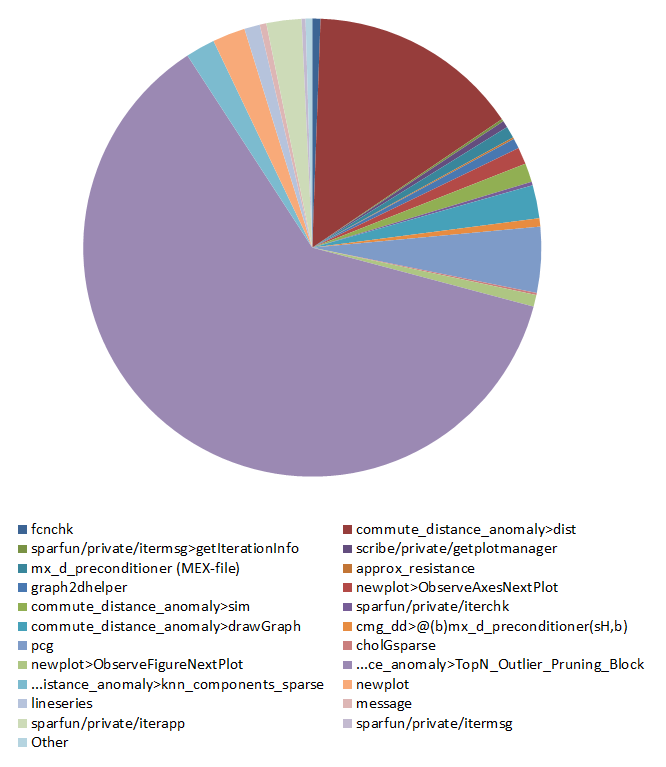
\includegraphics[width=0.8\textwidth]{profiling/original/testCD-profile}
\end{figure}

\subsection{Results}
\begin{figure}[H]
	\centering
	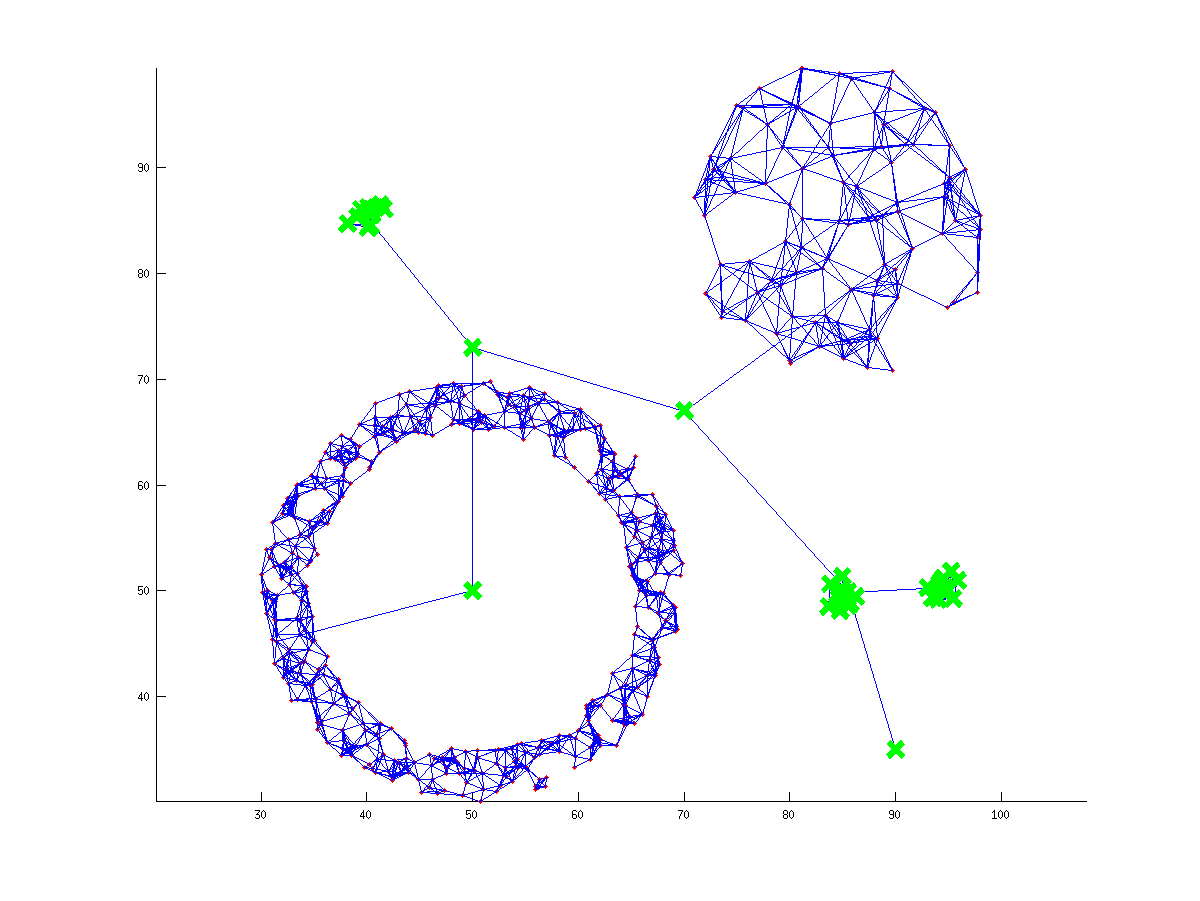
\includegraphics[width=0.8\textwidth]{profiling/original/testCD}
\end{figure}

% testCDST
\section{Data set 2}

\subsection{Data set summary}

\subsection{MATLAB execution profile}
\begin{figure}[H]
	\centering
	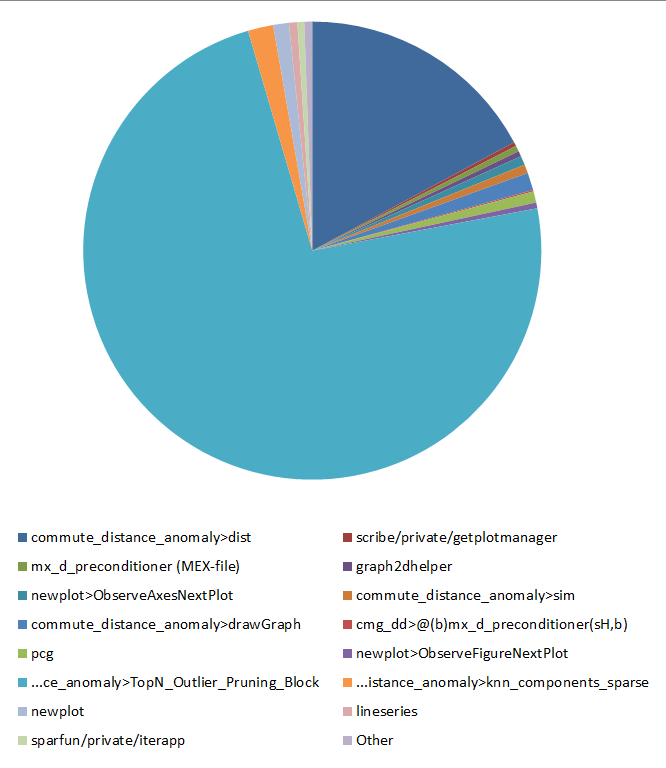
\includegraphics[width=0.8\textwidth]{profiling/original/testCDST-profile}
\end{figure}

\subsection{Results}
\begin{figure}[H]
	\centering
	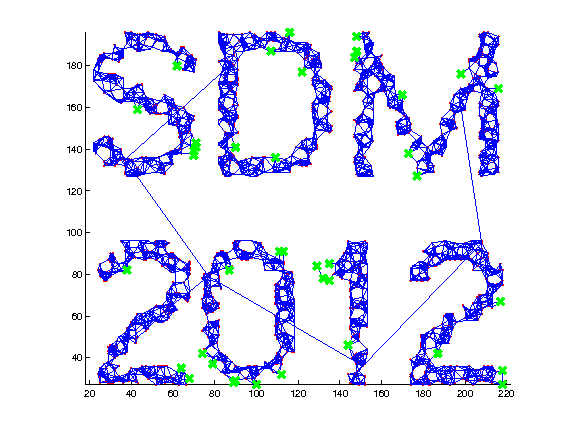
\includegraphics[width=0.8\textwidth]{profiling/original/testCDST}
\end{figure}

% testCDST2
\section{Data set 3}

\subsection{Data set summary}

\subsection{MATLAB execution profile}
\begin{figure}[H]
	\centering
	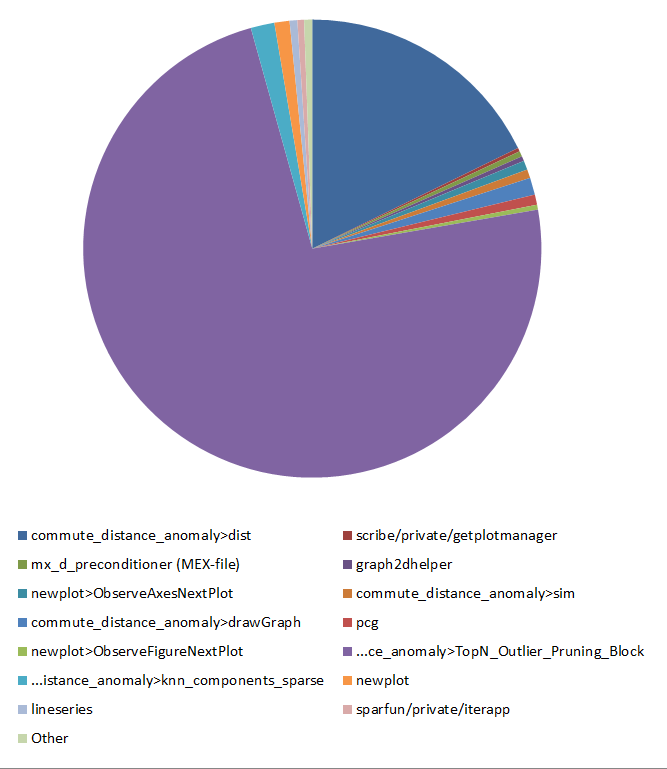
\includegraphics[width=0.8\textwidth]{profiling/original/testCDST2-profile}
\end{figure}

\subsection{Results}
\begin{figure}[H]
	\centering
	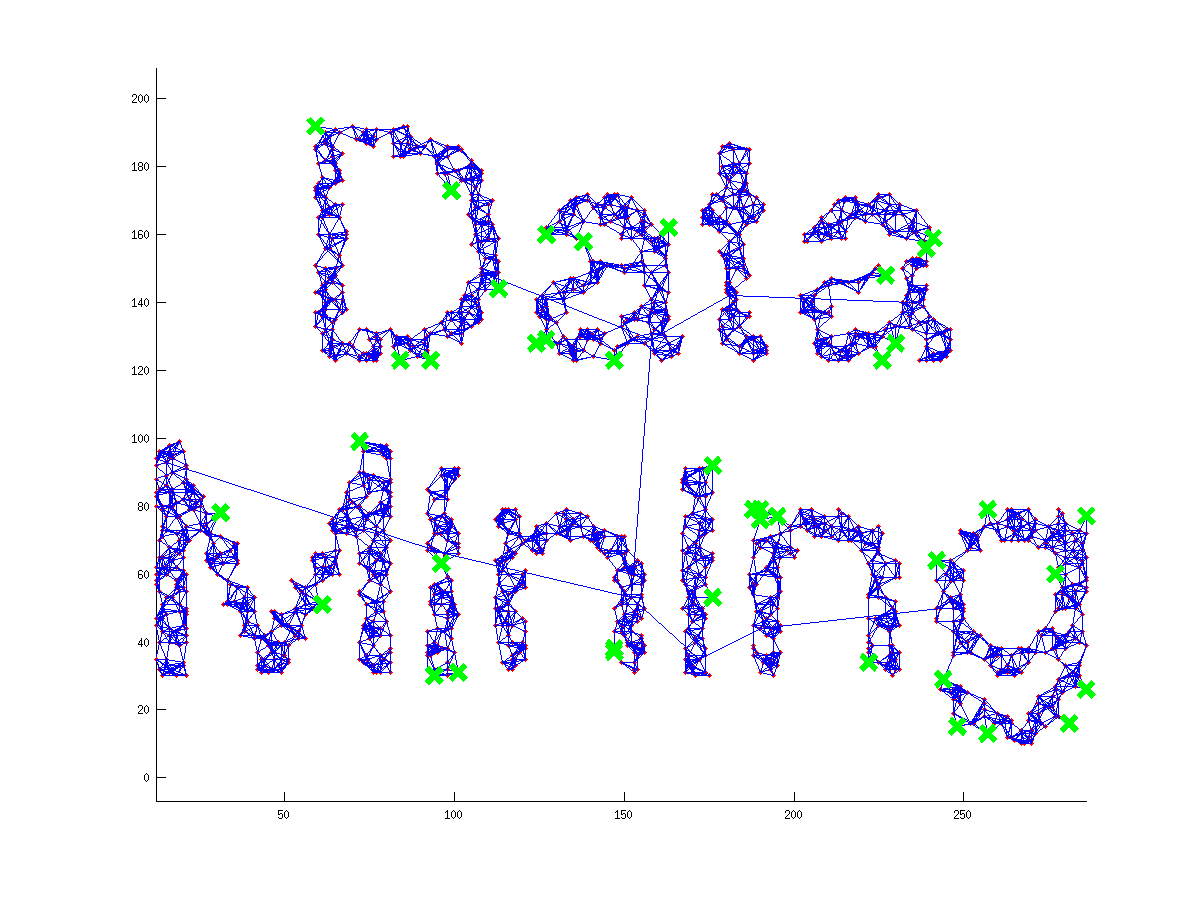
\includegraphics[width=0.8\textwidth]{profiling/original/testCDST2}
\end{figure}

% testCDST3
\section{Data set 4}

\subsection{Data set summary}

\subsection{MATLAB execution profile}
\begin{figure}[H]
	\centering
	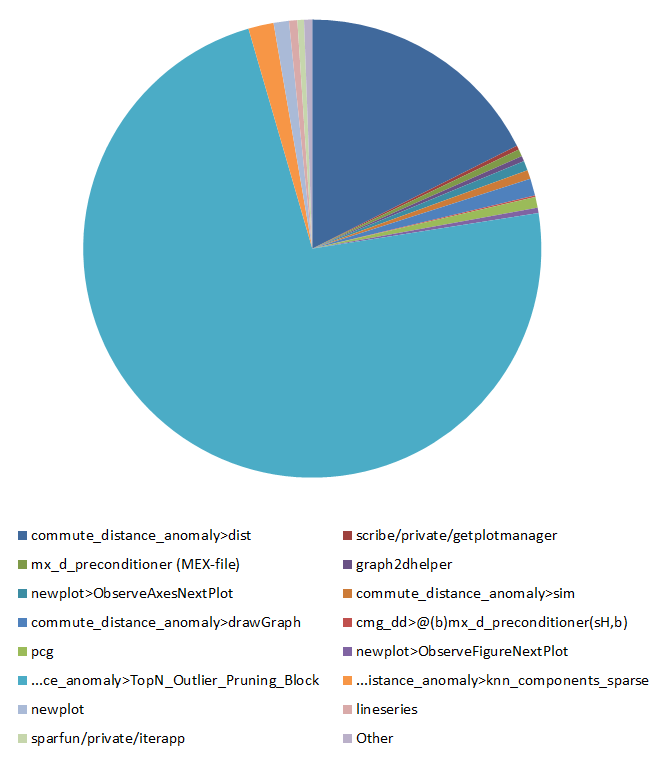
\includegraphics[width=0.8\textwidth]{profiling/original/testCDST3-profile}
\end{figure}

\subsection{Results}
\begin{figure}[H]
	\centering
	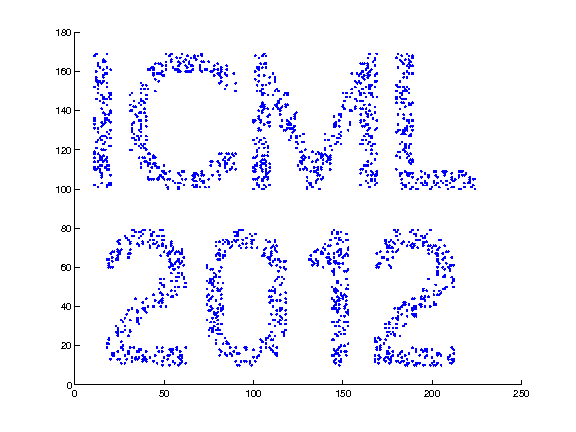
\includegraphics[width=0.8\textwidth]{profiling/original/testCDST3}
\end{figure}

% testoutrank
\section{Data set 5}

\subsection{Data set summary}

\subsection{MATLAB execution profile}
\begin{figure}[H]
	\centering
	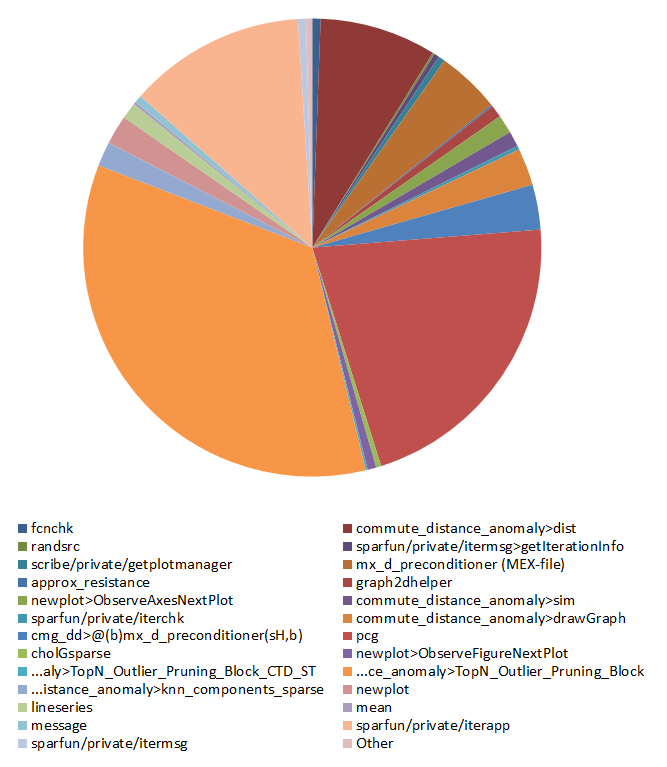
\includegraphics[width=0.8\textwidth]{profiling/original/testoutrank-profile}
\end{figure}

\subsection{Results}
\begin{figure}[H]
	\centering
	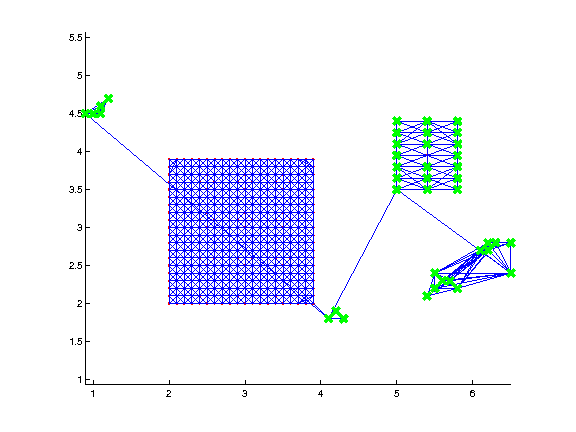
\includegraphics[width=0.8\textwidth]{profiling/original/testoutrank}
\end{figure}

% spam
\section{Data set 6}

\subsection{Data set summary}

\subsection{MATLAB execution profile}
\begin{figure}[H]
	\centering
	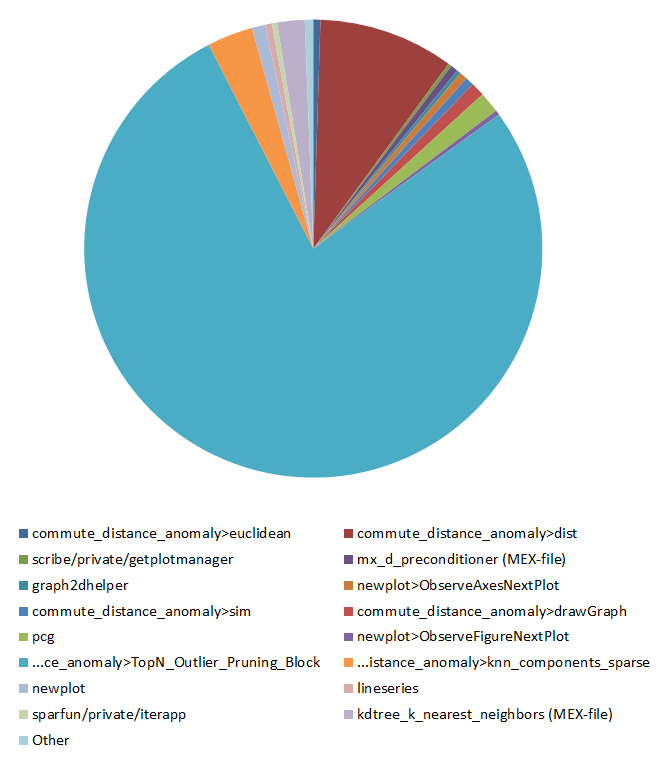
\includegraphics[width=0.8\textwidth]{profiling/original/spam-profile}
\end{figure}

\subsection{Results}
\begin{figure}[H]
	\centering
	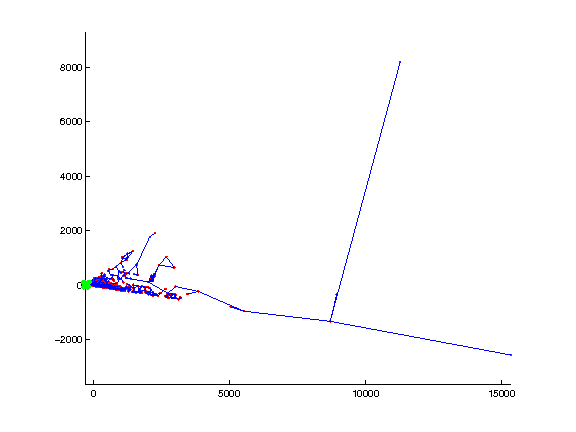
\includegraphics[width=0.8\textwidth]{profiling/original/spam}
\end{figure}

% PERFORMANCE BOTTLENECK
\subsection{Performance Bottleneck}
\label{sec:algorithmPerformanceBottleneck}
From observations of the results of the algorithm profiling, it was observed 
that the performance of the `anomaly detection using commute-distance' 
algorithm is bottle-necked significantly by a function named 
\verb+TopN_Outlier_Pruning_Block+. The MATLAB code for this function can be 
found in \hyperref[apdx:matlabCode]{Appendix~\ref{apdx:matlabCode}}. Analysis of
this function, as well as discussions with \citeauthor{Khoa:2012} revealed that
the algorithm was originally devised by \citeauthor{Bay:2003} and published in
the paper \citetitle{Bay:2003}. The general steps of the algorithm are described
in \hyperref[algm:TopNOutlierPruningBlock]
{Algorithm~\ref{algm:TopNOutlierPruningBlock}}.

\begin{algorithm}[t]
\caption{TopN\_Outlier\_Pruning\_Block}
\label{algm:TopNOutlierPruningBlock}

\LinesNumbered

\SetKwInput{InputK}{k}
\SetKwInput{InputN}{N}
\SetKwInput{InputD}{Data}
\SetKwInOut{OutputO}{outliers}

\InputK{the number of nearest neighbors}
\InputN{the number of outliers to return}
\InputD{a set of examples in random order}
\OutputO{a set of outliers}

\SetKwData{varB}{b}
\SetKwData{Block}{block}
\SetKwData{Cutoff}{cutoff}
\SetKwData{varD}{d}
\SetKwData{Data}{Data}
\SetKwData{varK}{k}
\SetKwData{varN}{N}
\SetKwData{Neighbours}{neighbours}
\SetKwData{varO}{o}
\SetKwData{Outliers}{outliers}
\SetKwData{Score}{score}

\SetKwFunction{Closest}{closest}
\SetKwFunction{Distance}{distance}
\SetKwFunction{GetNextBlock}{getNextBlock}
\SetKwFunction{MaxDist}{maxDist}
\SetKwFunction{Min}{min}
\SetKwFunction{Top}{top}

\Begin{
	$\Cutoff \longleftarrow 0$\tcp*[l]{set the cutoff for pruning to $0$}
	$\Outliers \longleftarrow \emptyset$\tcp*[l]{initialize to the empty set}
	\BlankLine
	\While(\tcp*[h]{load a block of examples from \varD}){$\Block \longleftarrow \GetNextBlock{\Data}$}{
		$\Neighbours(\varB) \longleftarrow \emptyset, \quad \forall \, \varB \in \Block$\;
		\BlankLine
		\ForEach{$\varD \in \Data$}{
			\ForEach{$\varB \in \Block \: : \: \varB \neq \varD$}{
				\If{$|\Neighbours(\varB)| < \varK \: \lor \: \Distance{\varB, \varD} < \MaxDist{\varB, \Neighbours(\varB)}$}{
					$\Neighbours(\varB) \longleftarrow \Closest{\varB, \Neighbours(\varB)} \cup \varD, \varK)$\;
					\If{$\Score(\Neighbours(\varB), \varB) < \Cutoff$}{
						$\Block \longleftarrow \Block \setminus \varB$\;
					}
				}
			}
		}
		\BlankLine
		$\Outliers \longleftarrow $\Top{$\Block \cup \Outliers$, $\varN$}\tcp*[l]{keep only the top n outliers}
		$\Cutoff \longleftarrow \Min_{\varO \in \Outliers}(\Score(\varO))$\tcp*[l]{the cutoff is the score of the weakest outlier}
	}
	\KwRet{\Outliers}\;
}
\end{algorithm}

In this algorithm, the \verb+score+ function can be any monotonically decreasing
function of the nearest neighbor distances such as the distance to the $k$th 
nearest neighbor, or the average distance to the $k$ neighbours \cite{Bay:2003}.

The main idea of the  nested loop algorithm is that for each example in the 
input set \verb+Data+, the algorithm keeps track of the closest neighbours found
so far. When an example's closest neighbours achieve a score lower than the 
\verb+cutoff+, the example is discarded because it can no longer be an outlier. 
As more examples are processed, the algorithm finds more extreme outliers and 
the \verb+cutoff+ increases along with pruning efficiency \cite{Bay:2003}.

In the worst case, the performance of the algorithm is very poor --- due to the 
nested loops, it could require $O(N^{2})$ distance computations and 
$O(\frac{N}{blocksize} \times N)$ data accesses. However, \citeauthor{Bay:2003} 
proved (through application of the algorithm to both real and synthetic data
sets) that the algorithm performs considerably better than the expected 
$O(N^{2})$ running time in the average case. The performance improvements over 
similar algorithms were attributed to the application of randomization and 
pruning techniques. The outlier pruning problem can be considered similar to the
problem of conducting a set of independent Bernoulli trials in which examples 
are analysed until $k$ examples within distance $d$ are found, or until the data
set is exhausted. \citeauthor{Bay:2003} proved that the number of trials 
expected to achieve $k$ examples within distance $d$ is given by:

\begin{equation}
\label{eqn:outlierPruneComplexity}
E[Y] \leq \frac{k}{\pi(\textbf{x})} + \Bigg(1 - \sum_{y=k}^{N} P(Y=y)\Bigg) \times N
\end{equation}

Where $\pi(x)$ is the probability that a random drawn example lies within 
distance $d$ of point $x$ and $P(Y=y)$ is the probability of obtaining the $k$th 
success on trial $y$.

The first term in \hyperref[eqn:outlierPruneComplexity]
{Equation~\ref{eqn:outlierPruneComplexity}} represents the number of distance 
computations to eliminate non-outliers, and does not depend on $N$. The second 
term represents the expected cost of outliers, and does depend on $N$, yielding 
an overall quadratic dependency to process $N$ examples in total. However, note 
that we typically set the program parameters to return a small and possibly 
fixed number of outliers. Thus the first term dominates and we obtain near 
linear performance \cite{Bay:2003}. More specifically, it was determined that 
the primary factor determining the scaling is how the cutoff changes as $N$ 
increases.

There are, however, some limitations of the aforementioned algorithm. 
Specifically:
\begin{enumerate}
\item The algorithm assumes that the data is in random order. If the data is not
in random order and is sorted then the performance can be poor.
\item The algorithm depends on the independence of examples. If examples are 
dependent in such a way that they have similar values (and will likely be in the
set of $k$ nearest neighbors) this can cause performance to be poor as the
algorithm may have to scan the entire data set to find the dependent examples.
\item The algorithm can perform poorly occurs when the data does not contain 
outliers.
\end{enumerate}
